\documentclass[a4paper]{article}
\usepackage[utf8]{inputenc}
\usepackage[spanish, es-tabla, es-noshorthands]{babel}
\usepackage[table,xcdraw]{xcolor}
\usepackage[a4paper, footnotesep=1.25cm, headheight=1.25cm, top=2.54cm, left=2.54cm, bottom=2.54cm, right=2.54cm]{geometry}
%\geometry{showframe}

%\usepackage{wrapfig}			%Wrap figure in text
\usepackage[export]{adjustbox}	%Move images
\usepackage{changepage}			%Move tables

\usepackage{tikz}
\usepackage{amsmath}
\usepackage{amsfonts}
\usepackage{amssymb}
\usepackage{float}
\usepackage{graphicx}
\usepackage{caption}
\usepackage{subcaption}
\usepackage{multicol}
\usepackage{multirow}
\usepackage{wrapfig}
\setlength{\doublerulesep}{\arrayrulewidth}
\usepackage{booktabs}
\usepackage[numbib, nottoc, notlot, notlof]{tocbibind}

\usepackage{hyperref}
\hypersetup{
    colorlinks=true,
    linkcolor=blue,
    filecolor=magenta,      
    urlcolor=blue,
    citecolor=blue,    
}

%Change Font Size

% #1 = size, #2 = text
\newcommand{\setparagraphsize}[2]{{\fontsize{#1}{6}\selectfont#2 \par}}		%Cambia el size de todo el parrafo
\newcommand{\setlinesize}[2]{{\fontsize{#1}{6}\selectfont#2}}				%Cambia el font de una oración

\newcommand{\note}[1]{
	\begin{center}
		\huge{ \textcolor{red}{#1} }
	\end{center}
}

%FONTS (IMPORTANTE): Compilar en XeLaTex o LuaLaTeX
\usepackage{anyfontsize}	%Font size
\usepackage{fontspec}		%Font type

\usepackage{etoolbox}
\usepackage{todonotes}

\newcommand{\observacion}[2]{  \ifnumequal{1}{#1}{ { \todo[inline,backgroundcolor=red!25,bordercolor=red!100]{\textbf{Observación: #2}} } }{  }  }

\setcounter{topnumber}{2}
\setcounter{bottomnumber}{2}
\setcounter{totalnumber}{4}
\renewcommand{\topfraction}{0.85}
\renewcommand{\bottomfraction}{0.85}
\renewcommand{\textfraction}{0.15}
\renewcommand{\floatpagefraction}{0.8}
\renewcommand{\textfraction}{0.1}
\setlength{\floatsep}{5pt plus 2pt minus 2pt}
\setlength{\textfloatsep}{5pt plus 2pt minus 2pt}
\setlength{\intextsep}{5pt plus 2pt minus 2pt}

\newcommand{\quotes}[1]{``#1''}
\usepackage{array}
\newcolumntype{C}[1]{>{\centering\let\newline\\\arraybackslash\hspace{0pt}}m{#1}}
\usepackage[american]{circuitikz}
\usetikzlibrary{calc}
\usepackage{fancyhdr}
\usepackage{units} 

\graphicspath{{../Control de posición no lineal/}{../Control de fuerza no lineal/}{../Control híbrido no lineal/}{../Referencias/}{../Deducción de modelo/}{../Conclusiones/}}

\pagestyle{fancy}
\fancyhf{}
\lhead{22.99 - Automación Industrial}
\rhead{Lambertucci, Londero B., Maselli, Mechoulam}
\rfoot{Página \thepage}

%Items con bullets y no cuadrados
\renewcommand{\labelitemi}{\textbullet }


\begin{document}

%%%%%%%%%%%%%%%%%%%%%%%%%
%		Caratula		%
%%%%%%%%%%%%%%%%%%%%%%%%%

\begin{titlepage}
\newcommand{\HRule}{\rule{\linewidth}{0.5mm}}
\center
\mbox{\textsc{\LARGE \bfseries {Instituto Tecnológico de Buenos Aires}}}\\[1.5cm]
\textsc{\Large 22.90  Automaci\'on Industrial}\\[0.5cm]


\HRule \\[0.6cm]
{ \Huge \bfseries Segundo Parcial}\\[0.4cm] 
\HRule \\[1.5cm]


{\large

\emph{Alumno:}\\
\vspace{3pt}

\begin{tabular}{lr} 	
\textsc{Lambertucci}, Guido Enrique  & 58009 \\

\end{tabular}

\vspace{20pt}

\emph{Profesores}\\
\textsc{Arias}, Rodolfo Enrique  \\
\vspace{3pt}
\textsc{Spinelli}, Mariano Tomás \\	
\vspace{3pt}
\textsc{Avogadro}, Federico Sofio \\	
\vspace{3pt}
\vspace{100pt}

\begin{tabular}{ll}

Presentado: & 18/11/21\\

\end{tabular}

}

\vfill

\end{titlepage}

%%%%%%%%%%%%%%%%%%%%%
%		Indice		%
%%%%%%%%%%%%%%%%%%%%%

\tableofcontents
\newpage

%%%%%%%%%%%%%%%%%%%%%
%		Informe		%
%%%%%%%%%%%%%%%%%%%%%
\section{Filtrado de Ruido}
Para el filtrado de ruido se opto por utilizar la funci\'on del paquete de vision de Peter Corke ``irank()''. 
Esto se debe a que el tipo de ruido que contamina la imagen es de tipo salt and pepper, caracterizado pro su alta amplitud. Justamente irank es una tecnica de filtrado no lineal que permite quitar este ruido sin perder definici\'on ni contaminar el promedio de la imagen con los valores  de los ruidos. Tambi\'en se consider\'o utilizar tecnicas como iopen o iclose pero al ver la efectividad de irank se opto por ella.

\begin{figure}[H]
	\centering
	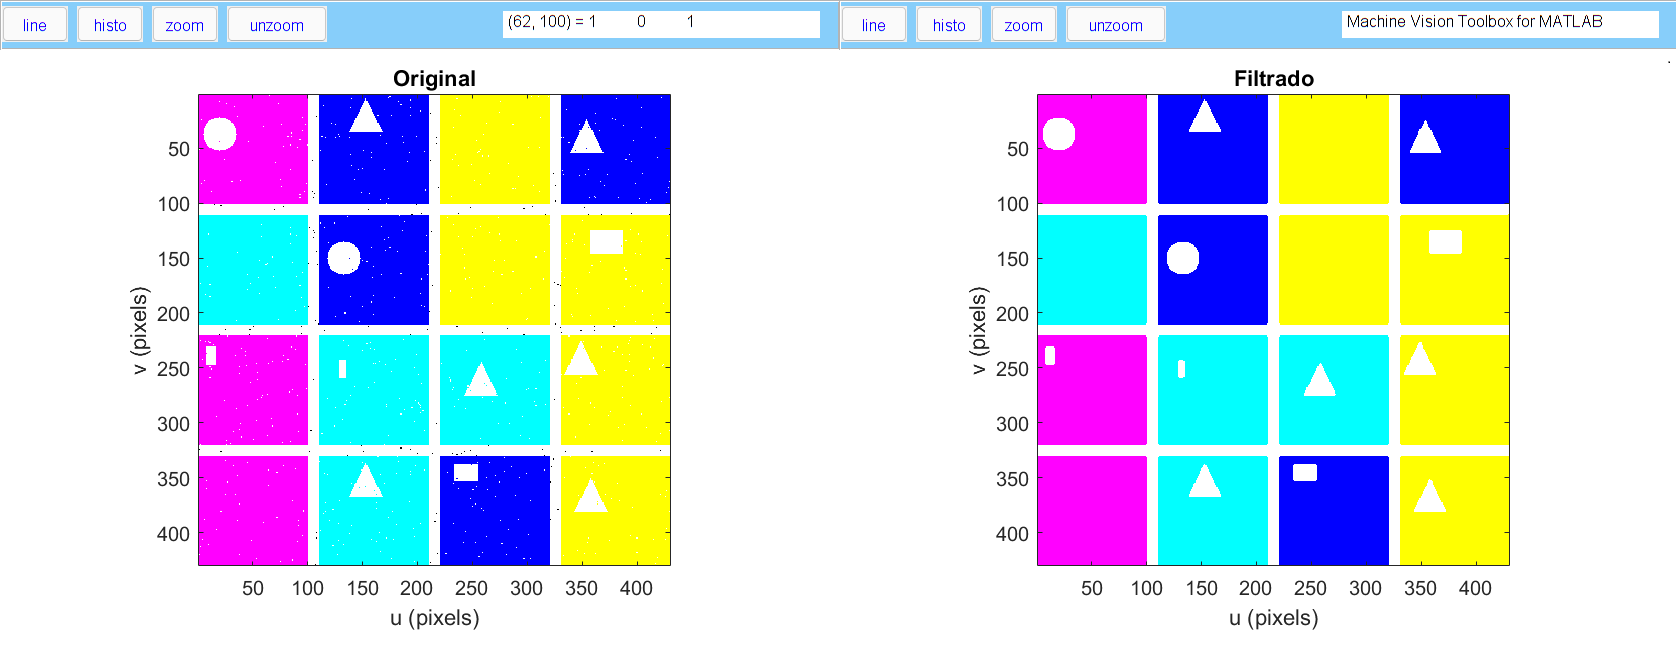
\includegraphics[width=0.8\linewidth]{Imagenes/comparacion_ruido.png}
	\caption{Comparativa original y ruido.}	
	\label{fig:or}
\end{figure}
Se puede observar el buen resultado de utilizar la funci\'on irank

\section{Idea de resoluci\'on}
Se separo el problema en 4 partes, primero filtro utilizando irnak, despues se busc\'o aislar en el cuadro principal en los 16 subcuadros.
Luego individualmente reconocer que forma hay en el subcuadro y finalmente cambiar los valores acorde a la siguiente regla.
\begin{itemize}
\item Si el cuadrante tiene un triángulo, elimine la componente roja de ese cuadrante.
\item Si el cuadrante tiene un rectángulo,  elimine la componente azul de ese cuadrante.
\item Si tiene un círculo, elimine la componente verde de ese cuadrante.
\end{itemize}
\section{Explicaci\'on de implementaci\'on}
\subsection{Main}
La función irank usa dos parametros, el orden y el structuring element, para el caso en particular se opt\'o por orden 4, con una ventana de 3x3. Para realizar el filtrado se tuvo que separar la imagen en RGB dado que irank no funciona con marcos RGB directamente.
Luego una vez filtrada la imagen se la imprime, y se procede al ``problema 2'' el cual es la separación en marcos individuales. Para esto se tomo del marco grande los submarcos teniendo en cuenta la la separación que tienen las imágenes entre si. Otra cosa a notar es que para el procesamiento de las formas se eligi\'o trabajar directamente en escala de grises ya que es mas sencillo.
As\'i queda separado en submarcos.
Despu\'es se taclea el problema de detectar la forma de las piezas, para esto se utilizar\'a la funci\'on iblobs.


Esto se logra utilizando las funciones ``filterDotsAndArea'' y ``detectForm''. Devolviendo un vector con las formas.
Luego se imprimen las formas de manera matricial y se cambian los colores originales por los propuestos por la consigna con la funci\'on ``changeCcolors'' y finalmente mostrar el marco final.

\lstinputlisting[language=Matlab]{./Codigo_separado/main.m}

Aqui se ve la salida del programa con la imagen filtrada y el reconocimiento de las figuras
\begin{figure}[H]
	\centering
	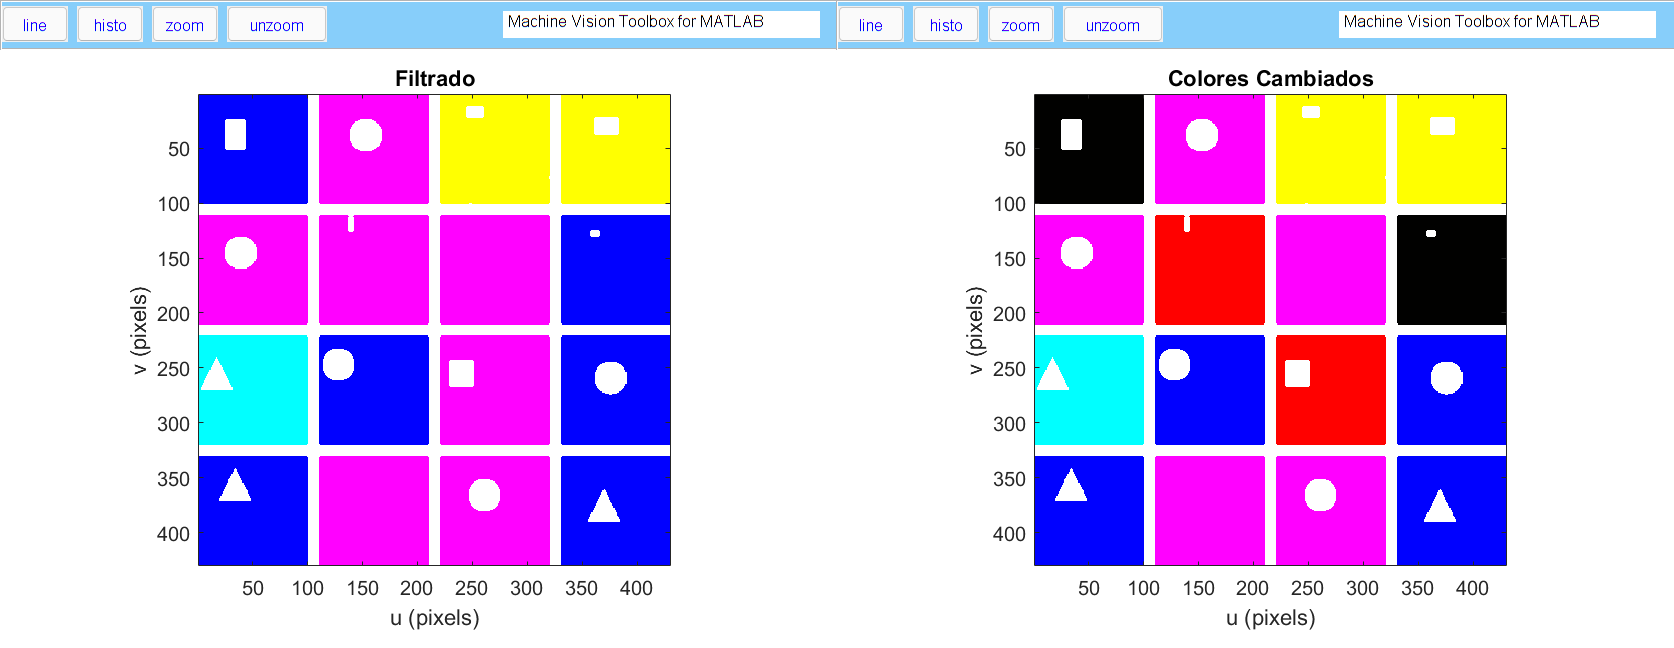
\includegraphics[width=0.8\linewidth]{Imagenes/Final.png}
	\caption{Comparativa filtrada y salida.}	
	\label{fig:fs}
\end{figure}

\begin{figure}[H]
	\centering
	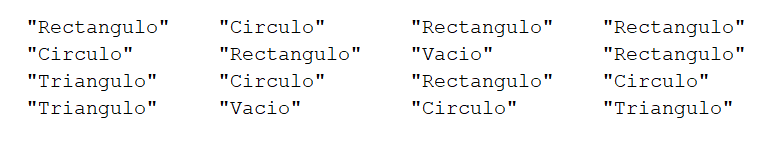
\includegraphics[width=0.8\linewidth]{Imagenes/comandwindow.png}
	\caption{Command window.}	
	\label{fig:cw}
\end{figure}
\subsection{FilterDotsAndArea}
Ahora explicar\'e la función ``filterDotsAndArea''.
Aqu\'i lo que se hace es fijarse las áreas, dado que siempre tiene un tamaño fijo los submarcos se puede saber el área si el marco esta vacío sin ningún tipo de ruido, lo que se hizo fue agregar unos thresholds para asegurarme de que aunque haya algo de ruido remanente todavía funcione. Para saber las areas se utiliza al función iblobs, esta devuelve un vector de blobs, lo que se hace aqui es sacar los blobs correspondientes a vaci\'io y unitarios.
\lstinputlisting[language=Matlab]{./Codigo_separado/filterDotsAndArea.m}
\subsection{detect form}
Pr\'oximo es el código de la función detect form:
La estrategia fue buscar cualidades características en las formas. Algo que se noto es que los círculos y triángulos todos mantienen su forma y \'area(teniendo en cuenta el ruido remanente). Y que los cuadrados no podr\'an tener un tamaño inferior a 5x5 y no mayor a 30x30.
La diferenciaci\'on de los triangulo se hace mediante su relación de aspecto. Debido a que siempre es un triangulo isósceles la relaci\'on $\frac{b}{a}$ ser\'a la misma. Luego se diferencian los rectángulos a partir de su área estimada. utilizando el ancho y alto del cuadrado se la estima y luego se la compara con la devuelta por iblobs. Para el circulo basta con que la relaci\'on $\frac{b}{a}$ sea aproximadamente 1.
Claro que esto ser\'ia un problema si se lo enfrenta con un cuadrado perfecto ya que su relación ba es 1 tambi\'en, pero estos son descartados antes ya que son catalogados como rectángulos antes gracias a la aproximaci\'on del \'area. Adicional mente cabe mencionar que el triangulo tambi\'en se lo podr\'ia diferenciar por la área, en vez de por la relaci\'on ba. Esta opción ser\'ia mas robusta antes triángulos de diversos ángulos internos. Pero debido a que en este problema esa situaci\'on no se da no se opt\'o por utilizar.
\lstinputlisting[language=Matlab]{./Codigo_separado/detect_form.m}
\subsection{print forms}
Print forms: recibe el vector de formas e imprime de manera estética la matriz de formas.
\lstinputlisting[language=Matlab]{./Codigo_separado/print_forms.m}
\subsection{change colors}
Finalmente queda la funci\'on change colors:
Esta recibe el marco filtrado original y el vector de formas. Y devuelve el marco con colores nuevos.
Utiliza el vector de formas para saber que forma est\'a mirando (acorde a los i, j) y así decide que hacer en el switch, sea caso rectángulo, triangulo, circulo o nada.
Se recorre cada bit preguntándose si es blanco o no, para saber si se multiplica por cero o no el valor.

\lstinputlisting[language=Matlab]{./Codigo_separado/change_colors.m}
\subsection{is not white}
La funci\'on is not white hace exactamente lo que el nombre sugiere. Recibe el valor de un bit RGB y devuelve 1 si no es blanco y 0 si es blanco.

\lstinputlisting[language=Matlab]{./Codigo_separado/is_not_white.m}

\end{document}